\subsection{Bộ dữ liệu}
Penn-Fudan Database for Pedestrian Detection and Segmentation \cite{dataset}\\
Bộ dữ liệu bao gồm các hình ảnh được lấy từ các cảnh xung quanh khuôn viên và đường phố đô thị. Đối tượng được quan tâm trong những hình ảnh này là người đi đường. Mỗi hình ảnh sẽ có ít nhất một người đi bộ trong đó.\\
Chiều cao của mỗi người đi bộ rơi vào khoảng [180,390] pixels. Và tất cả người đi bộ được dán nhãn đều có hướng thẳng đứng.\\
Tổng cộng bao gồm 170 hình ảnh và 345 người đi bộ được dán nhãn trong bộ dữ liệu này.

\begin{figure}[h!]
    \centering
    \subfloat[\centering Hình ảnh với ground truth box]{{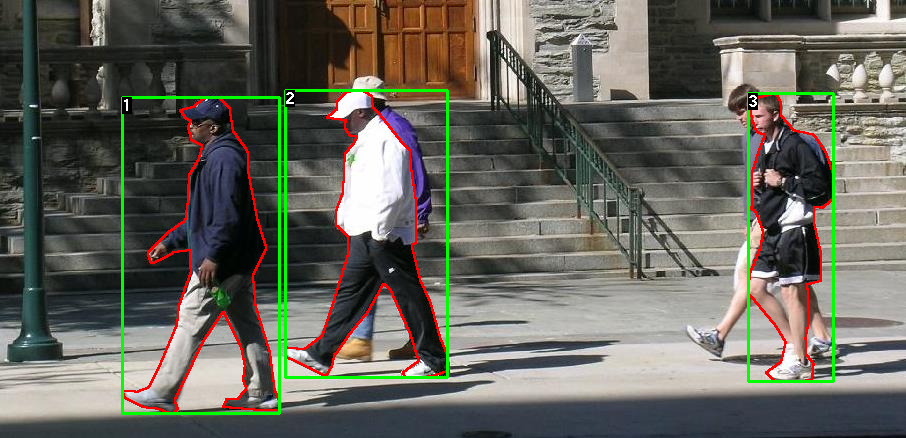
\includegraphics[width=7cm]{graphics/PennPed00015_1.png} }}%
    \qquad
    \subfloat[\centering Mask của hình ảnh]{{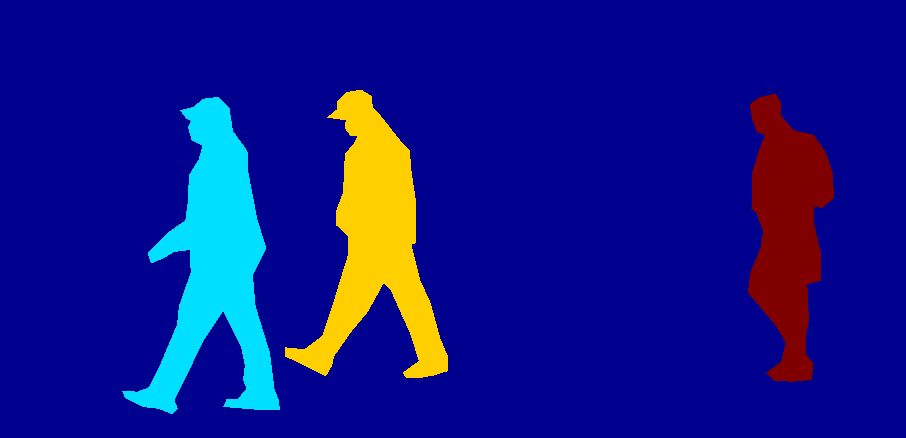
\includegraphics[width=7cm]{graphics/PennPed00015_2.png} }}
    \caption{Một ví dụ trong bộ dữ liệu}
    \label{fig:example}
\end{figure}